\section{Câu 9}
Cho một tín hiệu cần xử lý ở dạng điện áp, có tầm thay đổi từ 40mV – 200mV.\\
a. Thiết kế mạch cho ngõ ra tầm 4mA – 20mA.\\
b. Lựa chọn OPAMP và các linh kiện cần thiết để mạch hoạt động. Lưu ý: xử lý các
thông số không lý tưởng của OPAMP. (Tham khảo datasheet)\\

\begin{center}
\textbf{Bài giải}
\end{center}

a. Để thiết kế mạch chuyển đổi tín hiệu điện áp sang dòng điện ta biểu diễn mối quan hệ giữa dòng điện và điện áp như hình bên dưới
\begin{figure}[H]
    \centering
    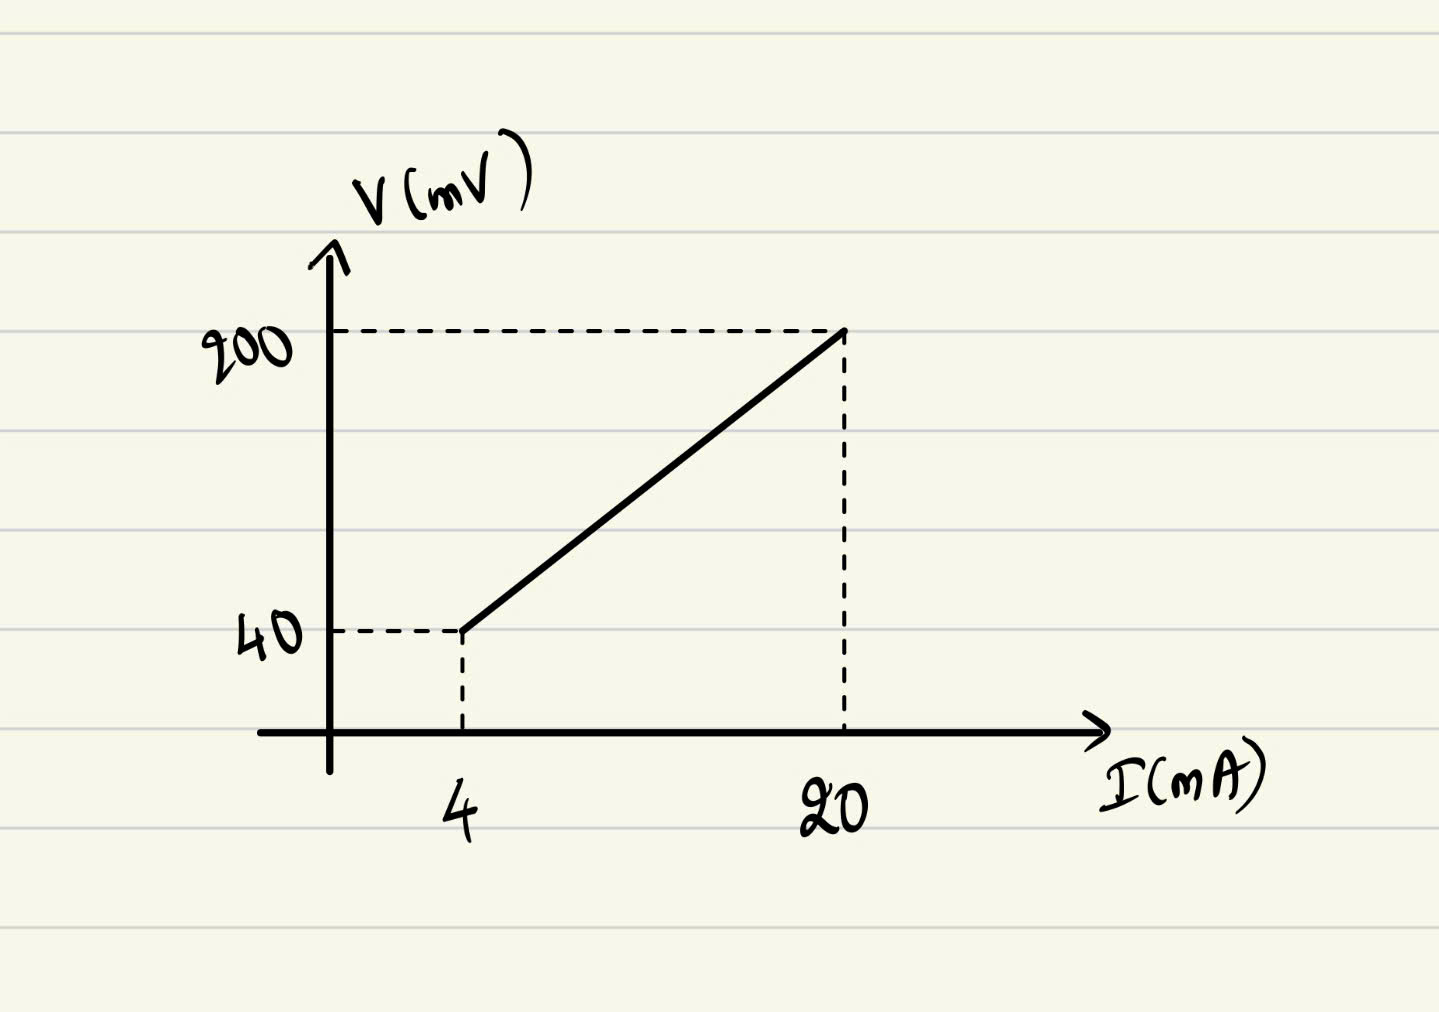
\includegraphics[scale=0.25]{image/C9_chart.png} 
\end{figure}
Từ hình trên ta có hệ phương trình:
\begin{equation*}
    \begin{cases}
        4 = 40\cdot a + b  \\
        20 = 200\cdot a + b\\
    \end{cases}
\end{equation*}
Giải hệ phương trình ta được:  
\begin{equation*}
    \begin{cases}
        a = 0.1 \\
        b = 0 \\
    \end{cases}
\end{equation*}
Vậy ta có phương trình mạch chuyển đổi điện áp sang dòng điện như hình bên dưới:\\
\begin{equation*}
    \boxed{I = 0.1V = \dfrac{V}{10\Omega}}
    \rightarrow \text{ Chọn } R_3 = 10\Omega
\end{equation*}
\\
b/ Ta phải chọn tỉ lệ
\begin{equation*}
    \dfrac{R_1}{R_5} = \dfrac{R_4}{R_3}
\end{equation*}
Chọn các điện trở khác đều là $10k\Omega$ để phù hợp với tỉ lệ và tận dụng thông số trở.\\
Chọn OPAMP LM358P vì các thông số tham khảo được: \\
- Băng thông: 1MHz, phù hợp cho mạch chuyển đổi tín hiệu chậm.\\
- Slew Rate: 0.3V/$\mu s$, phù hợp cho mạch so sánh và chuyển mạch chậm.\\
- Độ trễ ngõ ra so với ngõ vào thấp, phù hợp cho mạch tạo xung ổn định.\\
- Vos (độ dịch chuyển ngõ vào): 2mV.\\
- Ib (dòng dịch chuyển ngõ vào): 2nA.\\
- Ios (dòng dịch chuyển bù ngõ vào): 20nA (max).\\
Mạch hoàn chỉnh như hình bên dưới:
\begin{figure}[H]
    \centering
    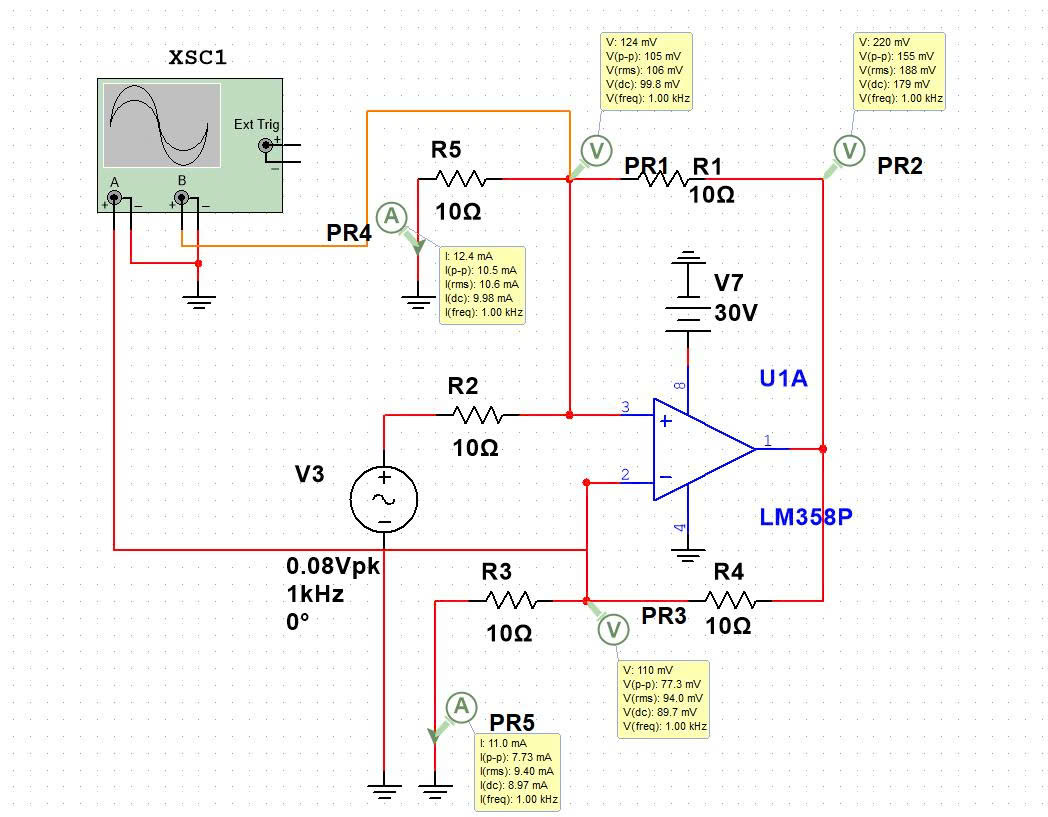
\includegraphics[scale=0.4]{image/C9.png}
\end{figure}

